\documentclass{article}
\PassOptionsToPackage{numbers,sort&compress}{natbib}
\usepackage[preprint]{neurips_2026}
\usepackage[utf8]{inputenc}
\usepackage[T1]{fontenc}
\usepackage{hyperref}
\usepackage{url}
\usepackage{booktabs,array,longtable}
\usepackage{microtype}
\usepackage[none]{hyphenat}
\usepackage{float}
\usepackage{tikz}
\usetikzlibrary{arrows.meta,calc}
\hypersetup{hidelinks,pdftitle={LearnLoop: A Stateful Agentic Platform for Adaptive Learning}}
\exhyphenpenalty=10000
\emergencystretch=2em
% Course proposal, not a conference submission. Keep the supplied style file
% unchanged; use named/nonanonymous preprint mode and the course notice.
\makeatletter
\renewcommand{\@noticestring}{COMP7608B Project Proposal}
\makeatother
\title{LearnLoop: A Stateful Agentic Platform\\for Adaptive Learning}
\author{COMP7608B Project Proposal}
\begin{document}
\maketitle
% The course explicitly requires no abstract.


\section{Group members}

\begin{tabular}{@{}>{\raggedright\arraybackslash}p{3.4in}>{\raggedright\arraybackslash}p{1.9in}@{}}
\toprule
\textbf{Name} & \textbf{Student ID} \\
\midrule
Fong Chi Ching & 3035299466 \\
\addlinespace[3pt]
Ching Nok Yee & 3035283572 \\
\addlinespace[3pt]
Lai Hok Lam Justin & 3036657081 \\
\addlinespace[3pt]
Zhou Yuxin & 3036791693 \\
\bottomrule
\end{tabular}

\section{Project objective}

We propose LearnLoop, an iterative learning platform for undergraduate and postgraduate students. Learners can upload their own course outlines, slides, notes, and readings, and set their learning goals. The platform will assess their understanding, choose suitable activities, and adjust a persistent learning plan as they progress. It will support different courses and continue the learning journey across sessions.

The main contribution is a source-grounded agent--environment loop: an LLM proposes an educational action, the runtime validates and executes it, and the resulting observation informs the next decision. The environment comprises learner responses, uploaded course resources, activity records, and the learning-plan database. Success requires appropriate interventions and verified state changes. ReAct informs the action--observation feedback \citep{ref2}.

LearnLoop will derive learning items and prerequisite relationships from uploaded materials. Their number and depth will reflect the documents' length, page count, structure, and topic coverage. It will maintain topic state and learner state, and provide explanations, diagnostic questions, and practice tasks through reusable mission templates. The initial implementation will prioritize uploaded materials, with broader topic exploration as a later extension.

\section{Motivation and challenges}

Students often receive course outlines, slides, and readings but are unsure where to start, which ideas matter most, or what they need to understand first. They may spend time reviewing familiar topics while overlooking gaps in their knowledge. A chatbot can explain a topic, but students still have to decide what to ask and keep track of their own progress.

We are developing LearnLoop to help students decide what to study next. It will organize their uploaded materials into a learning path, check what they understand, and offer practice or explanations where they need help. By remembering earlier attempts, it can revisit difficult topics and adjust the plan over time. Research on intelligent tutoring systems supports investigating this approach \citep{ref3}. We will evaluate whether LearnLoop selects useful activities and helps students navigate their materials more confidently.

The main challenges are recognizing a lasting misunderstanding rather than a temporary mistake, finding reliable support in the uploaded materials, and keeping an accurate record of progress. We will check assessment evidence before updating the learner's state, allow the system to express uncertainty, and limit repeated attempts when tools fail. Missions and rewards will support the learning tasks, while progress will depend on demonstrated understanding. We will assess learning and motivation separately, as suggested by research on gamification \citep{ref4}.

\section{Potential solutions}

\subsection{Agent roles and execution architecture}

LearnLoop will use three specialized roles within one shared LangGraph execution graph. The Teaching Agent identifies learning needs and chooses the next activity. The Assessment Agent checks responses against rubrics and returns evidence, misconceptions, and uncertainty. The Gamification Agent presents approved activities as missions while preserving their objectives and assessment criteria. Typed handoffs make their communication inspectable, and the shared runtime validates tool execution and state changes. Figure 1 shows the architecture.


\begin{figure}[H]
\centering
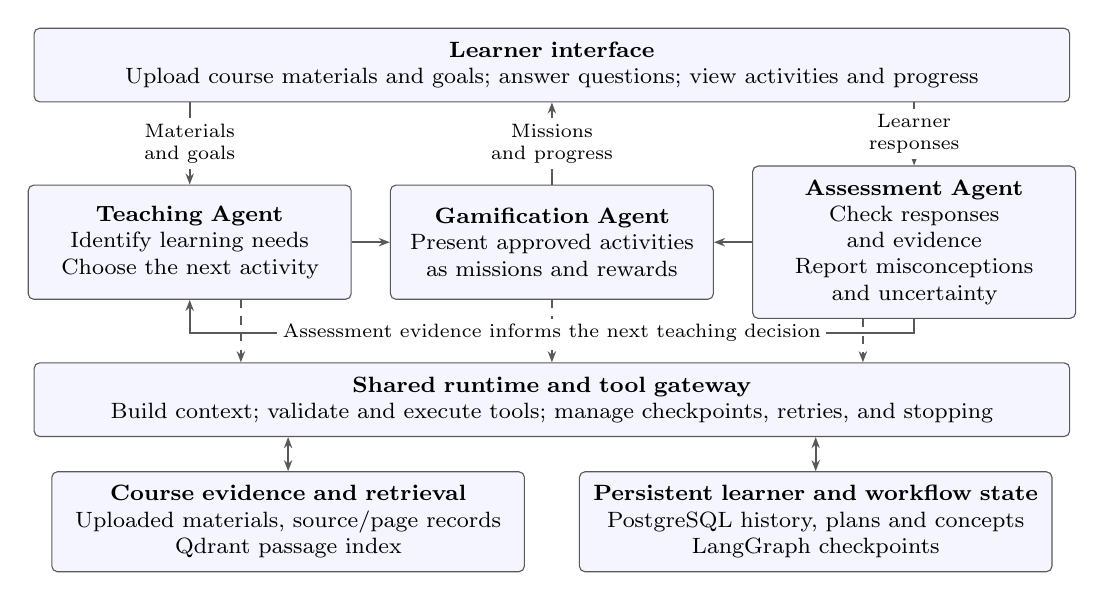
\begin{tikzpicture}[
  font=\footnotesize,
  box/.style={draw=black!65, rounded corners=2pt, align=center, inner sep=5pt, fill=blue!4},
  agent/.style={box, text width=3.75cm, minimum height=1.45cm},
  flow/.style={-{Stealth[length=4pt]}, thick, draw=black!65},
  label/.style={font=\scriptsize, fill=white, inner sep=2pt, align=center}
]
\node[box, text width=12.8cm] (ui) at (0,.25) {\textbf{Learner interface}\\Upload course materials and goals; answer questions; view activities and progress};
\node[agent] (teach) at (-4.6,-2) {\textbf{Teaching Agent}\\Identify learning needs\\Choose the next activity};
\node[agent] (game) at (0,-2) {\textbf{Gamification Agent}\\Present approved activities\\as missions and rewards};
\node[agent] (assess) at (4.6,-2) {\textbf{Assessment Agent}\\Check responses and evidence\\Report misconceptions and uncertainty};
\draw[flow] (ui.south -| teach.north) -- node[label] {Materials\\and goals} (teach.north);
\draw[flow] (game.north) -- node[label] {Missions\\and progress} (ui.south);
\draw[flow] (ui.south -| assess.north) -- node[label] {Learner\\responses} (assess.north);
\draw[flow] (teach.east) -- (game.west);
\draw[flow] (assess.west) -- (game.east);
\draw[flow] (assess.south) -- (4.6,-3.15) -- (-4.6,-3.15) -- (teach.south);
\node[box, text width=12.8cm] (run) at (0,-4.0) {\textbf{Shared runtime and tool gateway}\\Build context; validate and execute tools; manage checkpoints, retries, and stopping};
\coordinate (teachtool) at ([xshift=.65cm]teach.south);
\coordinate (assesstool) at ([xshift=-.65cm]assess.south);
\draw[flow,dashed] (teachtool) -- (run.north -| teachtool);
\draw[flow,dashed] (assesstool) -- (run.north -| assesstool);
\draw[flow,dashed] (game.south) -- (run.north);
\node[label] at (0,-3.15) {Assessment evidence informs the next teaching decision};
\node[box, text width=5.65cm] (retrieval) at (-3.35,-5.55) {\textbf{Course evidence and retrieval}\\Uploaded materials, source/page records\\Qdrant passage index};
\node[box, text width=5.65cm] (state) at (3.35,-5.55) {\textbf{Persistent learner and workflow state}\\PostgreSQL history, plans and concepts\\LangGraph checkpoints};
\draw[flow, {Stealth[length=4pt]}-{Stealth[length=4pt]}] (run.south -| retrieval.north) -- (retrieval.north);
\draw[flow, {Stealth[length=4pt]}-{Stealth[length=4pt]}] (run.south -| state.north) -- (state.north);
\end{tikzpicture}
\caption{LearnLoop agent roles and shared execution infrastructure. Dashed arrows denote tool calls through the shared runtime, which validates learner-state changes.}
\label{fig:architecture}
\end{figure}


Before each model call, the context builder selects the current objective, relevant learner history, source passages, and tool schemas. Retrieval supplies course evidence for generated explanations \citep{ref5}. The builder preserves source references, limits irrelevant history, and refreshes changed records.

\subsection{Observation decision execution and verification}

Each cycle observes the learner's response, selects an action, validates and executes a tool, and checks the result. New evidence can change the next decision. The runtime then continues, pauses for the learner, or stops within its execution limits. Appendix A gives the detailed workflow.

\subsection{Example adaptive episode}

A learner claims that retrieval updates a language model's weights. Assessment identifies a possible misconception, and teaching selects a diagnostic question supported by the course materials. The runtime assigns it and pauses for an answer. A correct answer with hints keeps developing status; two distinct independent successes can support advancement. Conflicting evidence prompts another diagnostic step. If source support is missing, the system reports the gap.

The agentic capability is selecting and executing actions in response to new evidence and changing learner state. Appendix A specifies the tools and runtime checks.

\subsection{Memory and learner state}

Working state will contain the current activity, selected evidence, pending action, tool results, and execution counters. Durable LangGraph checkpoints will preserve paused or interrupted cycles. Across sessions, PostgreSQL will store learner assessment history, preferences, plans, concept relationships, and source records. Qdrant will index course passages for retrieval, while PostgreSQL will remain the authoritative learner record.

Each concept record will contain a status, assessment IDs, misconception candidates, hint use, and review dates. Knowledge tracing motivates updating learner estimates from successive responses \citep{ref6}; our prototype will use explicit evidence rules rather than implement its probabilistic model. Statuses will be unassessed, developing, demonstrated, and review\_due. Advancement will require two distinct rubric-passing responses without hints, sufficient source support, and no unresolved conflicting evidence. This is a prototype policy to evaluate, not a validated mastery threshold. Scheduled review moves demonstrated to review\_due; unsuccessful review returns it to developing while preserving earlier evidence.

Assessment outputs will be candidate evidence. The runtime will validate activity identity, source references, required fields, and transition rules before committing changes. Records will retain owner, course, source, timestamp, and rubric version; reads will filter scope and freshness, and corrections will preserve an audit history. Reusing feedback in later decisions is informed by Reflexion \citep{ref7}, but learner evidence will remain distinct from agent self-reflection. Versioned diagnostic-remediation and source-grounded-assessment procedures will be loaded with relevant rubrics and templates. These procedures guide actions; tools perform them.

\subsection{Runtime control and recovery}

Pydantic schemas and an allowlisted tool gateway will check syntax, field types, ownership, resource existence, and operation preconditions. Semantic assessment will be evaluated separately because schema-valid output may still be wrong. Uploaded passages and learner responses will be treated as task data, with their provenance preserved, rather than as runtime instructions.

Each cycle will initially allow at most eight model calls, two attempts per transient read failure, and a 60-second execution deadline, excluding time awaiting the learner. These configurable limits will be recorded and tuned using development cases. A malformed proposal permits one repair within the same budget. Missing learner input causes a checkpointed pause; unsupported evidence or exhausted limits produces a clear fallback and a resumable progress record.

Mutating operations will use stable operation IDs, database transactions, and expected state versions. After a timeout or restart, the runtime will check whether a write committed before retrying, preventing duplicate activities or mastery updates. Traces will record selected context IDs, concise decision summaries, proposed and executed actions, tool observations, state differences, time, and cost. They will support failure localization without requiring hidden model reasoning.

\subsection{Implementation and trade offs}

A Next.js/React interface will display activities and progress; a FastAPI backend will run the shared LangGraph workflow. OpenRouter will provide hosted model access, with model identifiers and generation settings pinned for each experiment. BAAI/bge-m3 embeddings and Qdrant will support retrieval, while PostgreSQL and Docker Compose will provide persistent storage and reproducible deployment. We will first implement and test one complete learning cycle, then persistence and recovery, and finally template-based gamification and experiments. Retrieved support does not guarantee correctness, and additional assessment calls may increase latency; both limitations will be measured.

\section{Experimental dataset description and evaluation plan}

\subsection{Data and scenario construction}

We will evaluate permitted COMP7608B materials as a sample uploaded course, while LearnLoop will support students' own courses. Learning items and prerequisite links will be reviewed, with document and page references preserved. If needed, we will use an approved or openly licensed corpus.

Interactive agent evaluation motivates our trajectory tests \citep{ref8}. We plan 60 multi-step scenarios: 20 development cases and 40 held-out test trajectories, each spanning three to five responses. Development cases will tune prompts and policies; test cases will remain fixed. Each case will specify initial state, objective, evidence, acceptable interventions, and state constraints. Response scripts will branch by objective and activity type, with shared probes across variants. Held-out questions and reference answers will be excluded from retrieval.

The 40 test trajectories will comprise eight cases each for persistent misconceptions, hint-dependent or ambiguous answers, conflicting evidence, later-session review, and execution failures. Responses will be authored and reviewed for conceptual accuracy; any model-assisted drafts will be checked before inclusion. Alternative valid interventions will be allowed by the rubric. Scripted trajectories will test system behavior and will not be interpreted as human learning gains.

\subsection{Baselines and experimental controls}

We will compare LearnLoop with (a) a fixed-sequence tutor and (b) a tutor that adapts using only the current exchange, without cross-session learner memory. All variants will share the materials, question bank, assessment rubric, model configuration, mission presentation, and per-cycle budgets. Each of the 40 test trajectories will be run three times per variant, yielding 360 trajectory runs. A matched single-agent variant will be a secondary experiment if resources permit; a comparison without gamification will be exploratory.

\subsection{Measures and review protocol}

\begin{tabular}{@{}>{\raggedright\arraybackslash}p{1.35in}>{\raggedright\arraybackslash}p{3.95in}@{}}
\toprule
\textbf{Measure} & \textbf{Definition or assessment} \\
\midrule
Adaptive decision quality & Human rating from 1--4 for instructional alignment, evidence use, and appropriateness of the next intervention. \\
\addlinespace[3pt]
Assessment quality & Mean absolute score error against reviewed rubrics; precision and recall for labeled misconception detection. \\
\addlinespace[3pt]
State reliability & Invalid transitions / attempted transitions; premature demonstration / demonstration updates; duplicate committed effects. \\
\addlinespace[3pt]
Workflow robustness & Successful recoveries / injected recoverable faults; supported completion / eligible trajectories; schema-valid proposals / proposals. \\
\addlinespace[3pt]
Operational performance & p50 and p95 cycle latency, timeout rate, and all model/tool attempts and token costs per completed cycle; cold and warm runs separated. \\
\bottomrule
\end{tabular}

Two reviewers will independently score 15 stratified test trajectories per variant from the first repeat. We will report weighted agreement and adjudicate disagreements. Remaining outputs will receive one human review and automated checks. Paired differences and uncertainty intervals will group repeats by scenario. Failure analysis will separate context, decision, tool, and state-update errors.

An optional consenting learner pilot will explore usability and pre/post performance; an uncontrolled pilot cannot establish causal gains. Deliverables will include runnable code, versioned scenarios, configuration, failure traces, and measured quality, reliability, latency, and cost \citep{ref1}.

\label{main:end}

\clearpage

\appendix

\section{Tool contracts and verification cases}

The following planned interfaces make the model--runtime boundary explicit. Every result will include status and evidence or a structured error. Identifiers must refer to authorized course, learner, or activity records.

\subsection{Learning cycle}

{\small
\begin{longtable}{@{}>{\raggedright\arraybackslash}p{0.8in}>{\raggedright\arraybackslash}p{4.5in}@{}}
\toprule
\textbf{Stage} & \textbf{LearnLoop behavior} \\
\midrule
\endhead
Observe & Load the learning goal, current response, relevant history, and available course evidence. \\
\addlinespace[3pt]
Decide & Select diagnosis, prerequisite review, explanation, practice, advancement, or a request for clarification. Return a typed proposal with objective and evidence IDs. \\
\addlinespace[3pt]
Execute & Validate the proposal, authorize the operation, and dispatch a permitted tool that retrieves evidence, assigns an activity, or revises the plan. \\
\addlinespace[3pt]
Verify & Check tool outcomes, source support, and update preconditions; commit validated changes and retain the observation. \\
\addlinespace[3pt]
Continue or stop & Rebuild context after an observation; pause for the learner, finish the cycle, or report a blocked action when evidence or execution budgets are exhausted. \\
\bottomrule
\end{longtable}
}

\subsection{Tool contracts}

{\small
\begin{longtable}{@{}>{\raggedright\arraybackslash}p{1.13in}>{\raggedright\arraybackslash}p{1.43in}>{\raggedright\arraybackslash}p{2.59in}@{}}
\toprule
\textbf{Tool} & \textbf{Input contract} & \textbf{Result and runtime checks} \\
\midrule
\endhead
{\footnotesize \texttt{retrieve\_evidence}} & {\footnotesize \texttt{course\_id}, \texttt{concept\_id}, \texttt{query}} & Source passages and page IDs; course scope and retrieval limits enforced. Empty results preserve the evidence gap. \\
\addlinespace[3pt]
{\footnotesize \texttt{load\_learner\_state}} & {\footnotesize \texttt{learner\_id}, \texttt{concept\_ids}} & Current records and versions; ownership checked before selected records enter context. \\
\addlinespace[3pt]
{\footnotesize \texttt{assess\_response}} & {\footnotesize \texttt{activity\_id}, \texttt{response}, \texttt{hint\_used}} & Rubric score, evidence IDs, misconception candidates, uncertainty; activity and source references validated. \\
\addlinespace[3pt]
{\footnotesize \texttt{assign\_activity}} & {\footnotesize \texttt{operation\_id}, \texttt{objective\_id}, \texttt{activity\_type}, \texttt{evidence\_ids}} & Persisted activity ID and status; supported objective, template and evidence required. Duplicate operation IDs return the original outcome. \\
\addlinespace[3pt]
{\footnotesize \texttt{revise\_plan}} & {\footnotesize \texttt{operation\_id}, \texttt{expected\_version}, \texttt{activity\_ids}, \texttt{review\_dates}} & New plan version; learner ownership, prerequisite constraints and prior commit checked transactionally. \\
\addlinespace[3pt]
{\footnotesize \texttt{record\_assessment}} & {\footnotesize \texttt{operation\_id}, \texttt{expected\_version}, \texttt{assessment\_id}, \texttt{candidate\_update}} & Committed evidence and concept status; transition preconditions enforced. The model cannot directly overwrite mastery. \\
\bottomrule
\end{longtable}
}

\subsection{Executable acceptance cases}

Hint-dependent success: a correct hinted answer is recorded but cannot independently support demonstrated status. Contradictory evidence: a later wrong answer preserves the earlier record and requests diagnosis rather than silently discarding it. Missing evidence: retrieval returns no suitable source and the cycle reports insufficient support. Resume: an answer to a pending question restores the activity and counters from a durable checkpoint. Retry safety: a timed-out plan write that already committed returns its original result after restart, with no duplicate activity. Budget exhaustion: the runtime stops and retains a progress record instead of continuing indefinitely.

\subsection{Limits of the initial study}

A reviewed concept graph reduces extraction risk but does not test autonomous curriculum discovery. Authored trajectories provide controlled coverage but simplify real learner behavior. Source-grounded LLM assessment can still misgrade responses; persistent errors and uncertain cases will therefore be reported explicitly. Gamification is a supporting interface feature whose educational benefit remains an exploratory question.

\begin{thebibliography}{8}

\bibitem{ref1}COMP7608B Teaching Group. Final Project Guideline and Project Proposal Guidelines. Course requirements supplied as COMP7608B\_LLM\_Project\_Guideline.md.

\bibitem{ref2}Yao, S., Zhao, J., Yu, D., Du, N., Shafran, I., Narasimhan, K., and Cao, Y. (2023). ReAct: Synergizing Reasoning and Acting in Language Models. International Conference on Learning Representations (ICLR). \href{https://arxiv.org/abs/2210.03629}{Source}.

\bibitem{ref3}Ma, W., Adesope, O. O., Nesbit, J. C., and Liu, Q. (2014). Intelligent tutoring systems and learning outcomes: A meta-analysis. Journal of Educational Psychology, 106(4), 901--918. \href{https://doi.org/10.1037/a0037123}{Source}.

\bibitem{ref4}Sailer, M., and Homner, L. (2020). The Gamification of Learning: A Meta-analysis. Educational Psychology Review, 32, 77--112. \href{https://doi.org/10.1007/s10648-019-09498-w}{Source}.

\bibitem{ref5}Lewis, P., et al. (2020). Retrieval-Augmented Generation for Knowledge-Intensive NLP Tasks. Advances in Neural Information Processing Systems, 33, 9459--9474. \href{https://arxiv.org/abs/2005.11401}{Source}.

\bibitem{ref6}Corbett, A. T., and Anderson, J. R. (1994). Knowledge tracing: Modeling the acquisition of procedural knowledge. User Modeling and User-Adapted Interaction, 4, 253--278. \href{https://doi.org/10.1007/BF01099821}{Source}.

\bibitem{ref7}Shinn, N., Cassano, F., Gopinath, A., Narasimhan, K., and Yao, S. (2023). Reflexion: Language Agents with Verbal Reinforcement Learning. Advances in Neural Information Processing Systems, 36. \href{https://papers.nips.cc/paper_files/paper/2023/hash/1b44b878bb782e6954cd888628510e90-Abstract-Conference.html}{Source}.

\bibitem{ref8}Liu, X., et al. (2024). AgentBench: Evaluating LLMs as Agents. International Conference on Learning Representations (ICLR). \href{https://arxiv.org/abs/2308.03688}{Source}.

\end{thebibliography}

\end{document}
